\subsection{Controller-Aware Generation and Final Objective}
\label{sec:controller-injection}

The fused controller vector 
\(\displaystyle \tilde{s} = \sum_{k=1}^K a_k\,s_k\in\mathbb{R}^d\) 
(where \(a_k=\exp(w_k)/\sum_{m}\exp(w_m)\) and \(w_k=g_\phi(s_k,\delta_k,c_k)\)) serves as a global conditioning signal for the transformer encoder.  X-Spanformer supports three fully differentiable injection pathways that bias computation at different stages of the network (Figure~\ref{fig:controller_injection_modes}).

\begin{figure}[H]
	\centering
	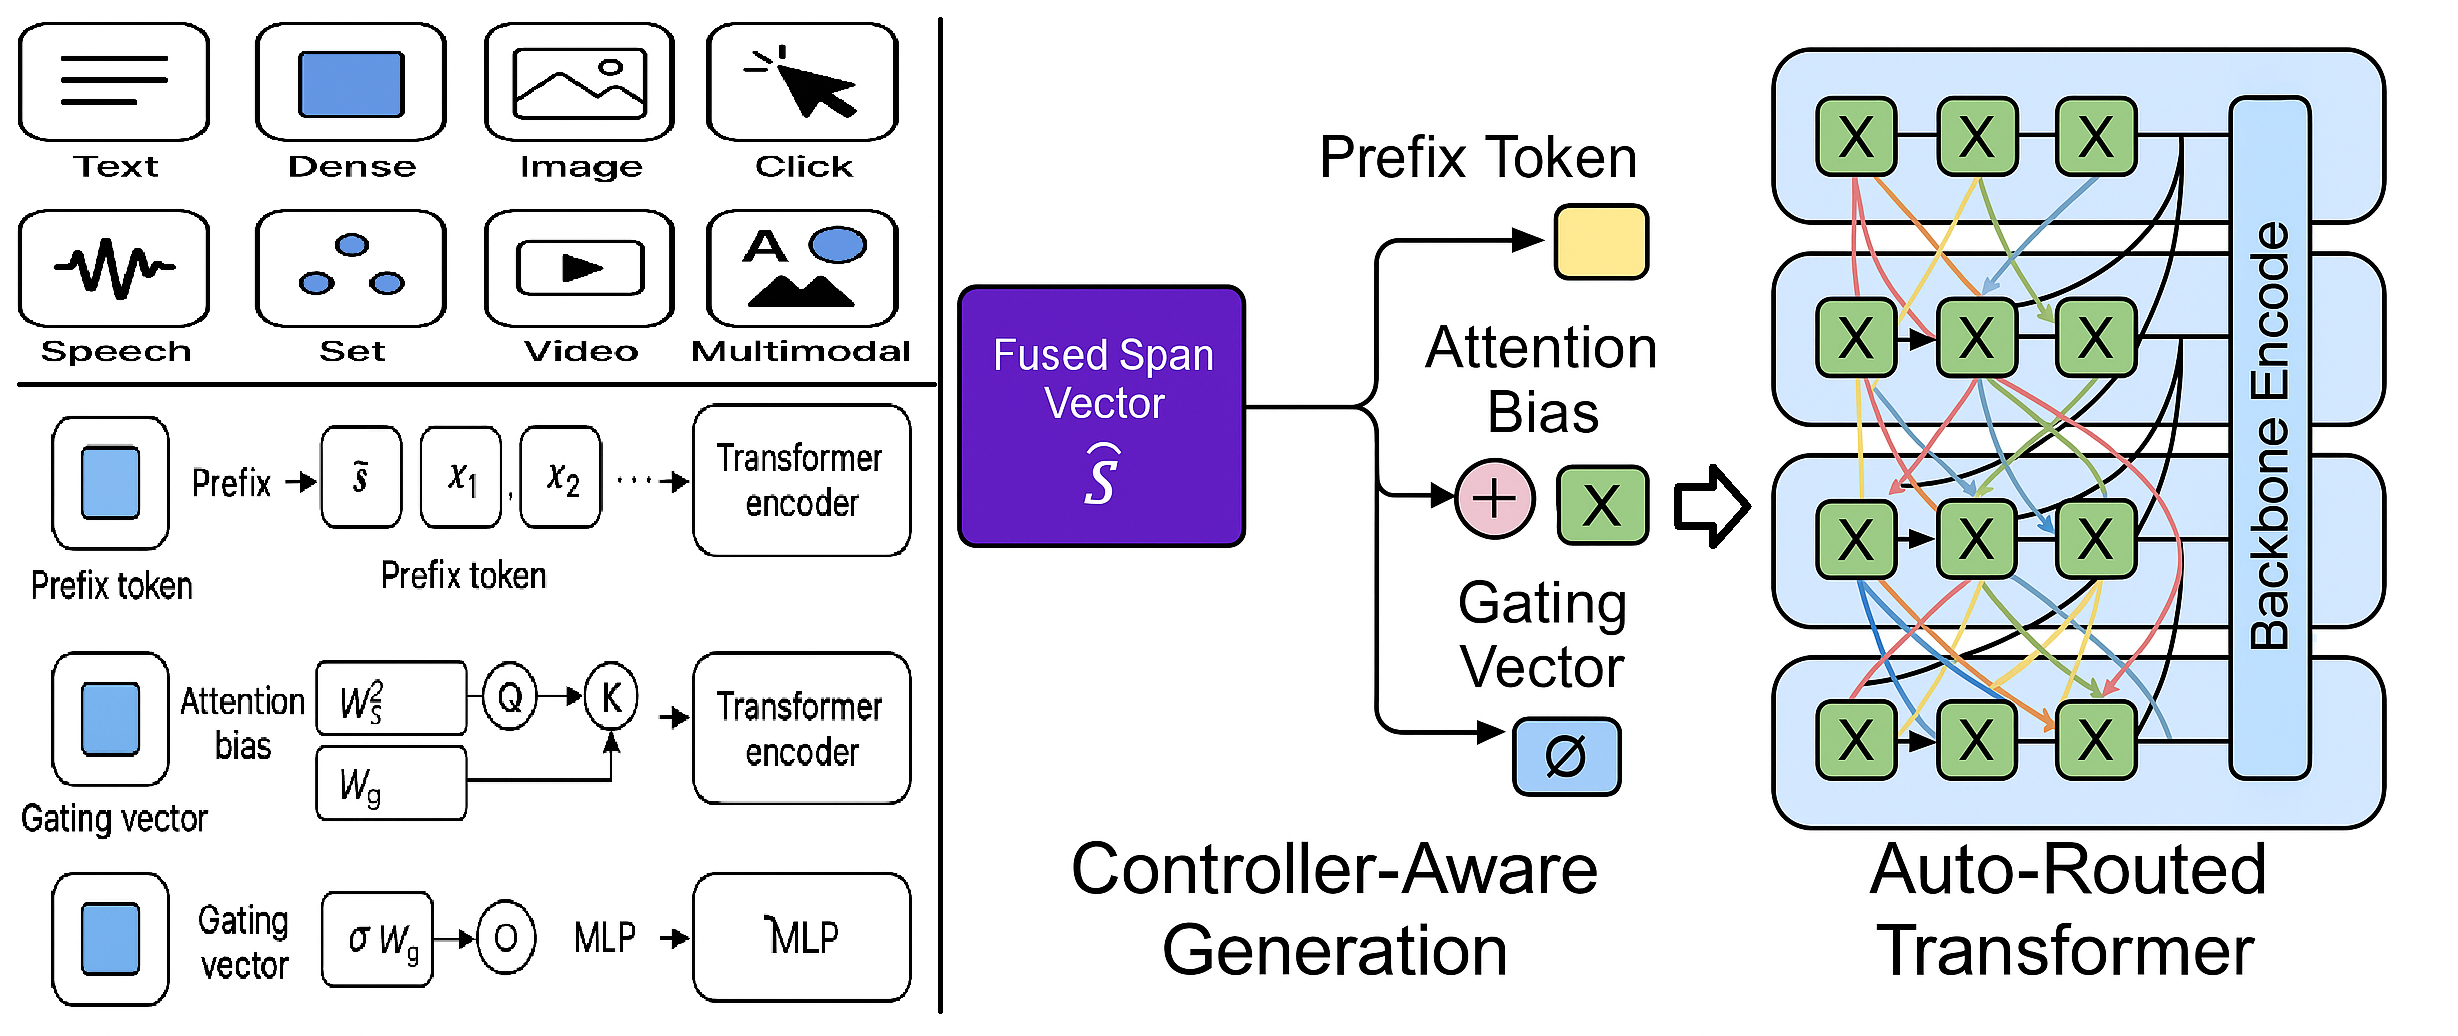
\includegraphics[width=0.92\textwidth]{figures/figure_5.png}
	\caption{Controller injection modes: prefix-token insertion, attention-bias adaptation, and gated FFN modulation.}
	\label{fig:controller_injection_modes}
\end{figure}

\subsubsection{Prefix-Token Injection}
We prepend \(\tilde{s}\) as a synthetic token at position 0:
\[
H' = \bigl[\tilde{s};\,h_1;\dots;h_T\bigr]\in\mathbb{R}^{(T+1)\times d}.
\]
A learned position embedding for index 0 ensures \(\tilde{s}\) participates in all attention heads from the first layer \cite{li2021prefix}. 

\subsubsection{Attention-Bias Injection}
We modify the attention logits by adding low-rank biases derived from \(\tilde{s}\):
\[
Q_i \;\leftarrow\; Q_i + W_Q\,\tilde{s},
\quad
K_j \;\leftarrow\; K_j + W_K\,\tilde{s},
\]
so that attention scores become 
\(\exp\bigl((Q_i + W_Q\tilde{s})^\top(K_j + W_K\tilde{s})\bigr)\).  
Here \(W_Q,W_K\in\mathbb{R}^{d\times d}\) learn to steer query and key subspaces \cite{hu2021lora}.  

\subsubsection{Gated-FFN Injection}
At each transformer layer, we modulate the feed-forward output by a span-conditioned gate:
\[
g = \sigma\bigl(W_g\,\tilde{s} + b_g\bigr)\in(0,1)^d,
\quad
h_i' = h_i + g \odot \mathrm{FFN}(h_i),
\]
where \(W_g\in\mathbb{R}^{d\times d}\), \(\sigma\) is sigmoid, and \(\odot\) denotes elementwise multiplication.  This gate adaptively amplifies or attenuates nonlinear transformations based on span context \cite{shazeer2017outrageously}.

\subsubsection{Semantic Routing Interpretation}
Injecting \(\tilde{s}\) as a dynamic, learned prompt parallels latent prompting and adapter routing frameworks (e.g.\ \cite{raffel2020exploring,liu2022pada,gupta2022molt}).  Unlike fixed metadata tags, our controller emerges from differentiable span selection, yielding semantically grounded routing signals.

\subsubsection{End-to-End Differentiability}
\begin{proposition}
	\label{prop:controller_diff}
	If each span embedding \(s_k=\mathrm{Pool}(x_{i_k:j_k})\) is a differentiable function of \(x\), and \(\tilde{s}\) is computed by
	\(\tilde{s}=\sum_k a_k s_k\) with \(a_k=\softmax(w_k)\), then for all three injection modes—prefix, bias, and gated-FFN—the final task loss \(\mathcal{L}\) is differentiable with respect to the span scorer parameters, pooling operator, and encoder parameters.
\end{proposition}
\begin{proof}
	We establish differentiability by showing that each injection mode creates a differentiable path from input \(x\) to task loss \(\mathcal{L}\).
	
	\textbf{Given assumptions:}
	\begin{enumerate}
		\item Each span embedding \(s_k = \mathrm{Pool}(x_{i_k:j_k})\) is differentiable in \(x\)
		\item Controller weights \(a_k = \softmax(w_k)\) where \(w_k\) are learnable parameters
		\item Fused controller \(\tilde{s} = \sum_{k=1}^K a_k s_k\)
	\end{enumerate}
	
	\textbf{Step 1:} Show \(\tilde{s}\) is differentiable in \(x\).
	Since \(s_k\) is differentiable in \(x\) by assumption, and \(a_k = \softmax(w_k)\) is differentiable in \(w_k\), we have:
	\[
	\frac{\partial \tilde{s}}{\partial x} = \sum_{k=1}^K a_k \frac{\partial s_k}{\partial x} + \sum_{k=1}^K s_k \frac{\partial a_k}{\partial w_k} \frac{\partial w_k}{\partial x}
	\]
	Both terms exist by the chain rule and differentiability assumptions.
	
	\textbf{Step 2:} Analyze each injection mode.
	
	\textit{Case 1 - Prefix injection:} \(H' = [\tilde{s}; h_1; \ldots; h_T]\)
	The augmented sequence passes through standard transformer attention:
	\[
	\frac{\partial \mathcal{L}}{\partial \tilde{s}} = \frac{\partial \mathcal{L}}{\partial H'} \frac{\partial H'}{\partial \tilde{s}}
	\]
	Since \(\frac{\partial H'}{\partial \tilde{s}} = [1; 0; \ldots; 0]\), gradients flow directly to \(\tilde{s}\).
	
	\textit{Case 2 - Attention bias:} \(Q_i \leftarrow Q_i + W_Q \tilde{s}\), \(K_j \leftarrow K_j + W_K \tilde{s}\)
	Attention scores become \(A_{ij} = \exp((Q_i + W_Q \tilde{s})^T(K_j + W_K \tilde{s}))\).
	\[
	\frac{\partial A_{ij}}{\partial \tilde{s}} = A_{ij} \left[ (K_j + W_K \tilde{s})^T W_Q + (Q_i + W_Q \tilde{s})^T W_K \right]
	\]
	This is well-defined since exponential and linear functions are differentiable.
	
	\textit{Case 3 - Gated FFN:} \(h_i' = h_i + g \odot \mathrm{FFN}(h_i)\) where \(g = \sigma(W_g \tilde{s} + b_g)\)
	\[
	\frac{\partial h_i'}{\partial \tilde{s}} = \frac{\partial g}{\partial \tilde{s}} \odot \mathrm{FFN}(h_i) = \sigma'(W_g \tilde{s} + b_g) \odot W_g \odot \mathrm{FFN}(h_i)
	\]
	Since \(\sigma\) is the sigmoid function, \(\sigma'\) exists everywhere.
	
	\textbf{Step 3:} Apply chain rule.
	In all cases, \(\frac{\partial \mathcal{L}}{\partial x} = \frac{\partial \mathcal{L}}{\partial \tilde{s}} \frac{\partial \tilde{s}}{\partial x}\) exists by composition of differentiable functions.
\end{proof}

\subsubsection{Final Objective}
Let \(\mathcal{L}_{\mathrm{task}}\) be the downstream loss (e.g.\ cross-entropy or contrastive).  The total training objective is
\[
\mathcal{L}
= \mathcal{L}_{\mathrm{task}}
+ \beta_1\,\mathcal{L}_{\mathrm{span}}
+ \beta_2\,\mathcal{L}_{\mathrm{ent}},
\]
where \(\beta_1,\beta_2\ge0\) balance structural supervision and entropy regularization.\footnote{Typical ranges: \(\beta_1\in[0.5,1.5]\), \(\beta_2<0.3\) after warmup. These ranges were empirically determined to ensure stable training dynamics and promote sparsity in the learned representations.}
